\chapter{The Control Structure} \label{chap:control}

The control Structure used is the one of ArduPlane, in hover, or tail-sitter mode, the ArduCopter stabilization system is used, while in airplane/fixed-wing mode, Arduplane's controllers are used. Both will be discussed and explained in the following sections.

\section{The Data Acquisition}

In order to control all the required variables, they must be available for the controller. The Pixhawk controller provides two redundant IMUs for this reason. Each of them runs an Extended Kalman Filter tracking 22 states\cite{kalman}\cite{kalmanArducopter}. Of the two running Kalman Filters, the one with smaller error estimation is used, and the estimated states are made available for the controllers.

\section{On Airplane Mode}

On Airplane mode, the aircraft is always moving forward, towards the $X$ axis, position control depends on defining a route and pointing the aircraft in order to remain on it.

\subsection{Roll and Pitch Control}

The roll and pitch control loops (seen on Figures \ref{fig:roll_loop} and \ref{fig:pitch_loop})) are responsible for keeping the aircraft on the desired orientations on the $X$ and $Y$ axis. Usually, pitch is controlled by turning the elevator up and down, while roll is controlled by the deflecting the ailerons. On this aircraft, however, there are only two control surfaces, such that the output of both controllers are summed ("mixed", as is usually said in the RC world) in order to control both axis at the same time.
While at first they look like a classical P+I+D controller, there are some small changes:

\begin{itemize}
\item There's a feedforward controller trying to cancel the current angular rates.
\item The Derivative and Integral terms and scaled to the airspeed, and the controller's output as well. This is because  as the aircraft moves faster, less deflection is necessary to displace the same amount of air, resulting in the same movement of the body.
\end{itemize}


The controller outputs are called AileronDemand and ElevatorDemand, and are the theoretical required input on each axis. Ardupilot works like this in order to abstract the possible airframes. The next code stage mixes these needs to get the proper output for the current airframe.
On an airplane, the outputs are only limited to the maximum and minimum possible outputs, on an aircraft like the one in this project, the outputs are summed and subtracted to get the correct outputs on each elevon.


\begin{figure}[H]
\centering
  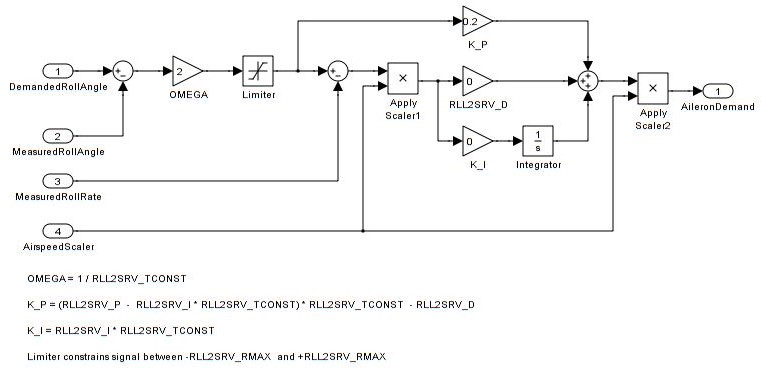
\includegraphics[width=\linewidth]{figs/roll_control_loop.jpg}
  \caption{Roll control loop. Source: ArduPilot}
  \label{fig:roll_loop}
\end{figure}

The transfer function for RollDemand is as follow:

\begin{equation}
D_{ail}(s) = \bigg(\frac{A_s(s) K_p s + A_s(s)^2(K_d s + K_i)}{s}\bigg)(\overline{R}(s) - R(s)) - A_s^2(K_D s + K_i)Rs
\end{equation}
\begin{equation}
R(s) = \Omega sat(R_{raw}(s))
\end{equation}

Where $R_{raw}(s)$ is the raw roll reading, $D_{ail}(s)$ is the aileron demand, $A_s(s)$ is an airspeed scaling value, $0 < A_s < 1$ (responsible for reducing the control outputs at higher speed, as most aerodynamical forces are proportional to the square of the airspeed), $K_d$ is a derivative term, $K_i$ is an integral term, $\overline{R}(s)$ is the Roll angle setpoint, and $R(s)$ is the current roll angle.


\begin{figure}[H]
\centering
  \includegraphics[width=\linewidth]{figs/PitchAP.jpg}
  \caption{Pitch control loop. Source: ArduPilot}
  \label{fig:pitch_loop}
\end{figure}

The transfer function for PitchDemand is similar:

\begin{equation}
D_{pit}(s) = \bigg(\frac{A_s(s) K_p s + A_s(s)^2(K_d s + K_i)}{s}\bigg)(\overline{P}(s) - P(s)) - A_s^2(K_D s + K_i)Ps
\end{equation}
\begin{equation}
P(s) = \Omega sat(P_{raw}(s)) + P_{2R}R(s)
\end{equation}

Where $P_{raw}(s)$ is the raw roll reading, $D_{pit}(s)$ is the aileron demand, $A_s(s)$ is the same airspeed scaling value, $K_d$ is the derivative term, $K_i$ is the integral term, $\overline{P}(s)$ is the Pitch angle setpoint, and $P(s)$ is the current pitch angle. Additionally, $P_{2R}R(s)$ is a term that attempts to cancel out the effect of banking the aircraft affecting the pitch.



\subsection{Yaw Control}
The Yaw Control loop controls the angle around the Z axis. This is usually used for landing only, and is not necessary on this aircraft on airplane mode. It can, however, be seen on Figure \ref{fig:yaw_loop}.
Like the D and I terms on the roll axis, the controller's output is again scaled with the square of the \textit{AirspeedScaler} factor.
%\todo{dafuq?}

\begin{figure}[H]
\centering
  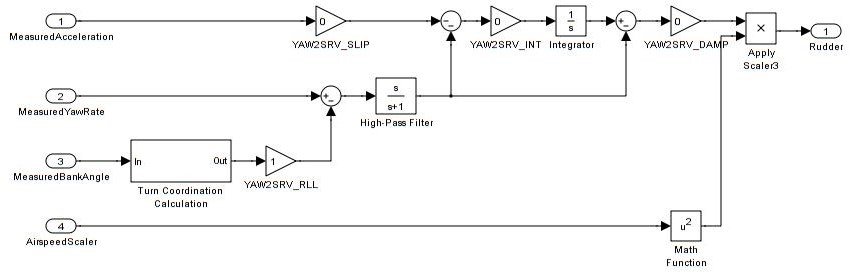
\includegraphics[width=\linewidth]{figs/yaw_control_loop.jpg}
  \caption{Yaw control loop. Source: ArduPilot}
  \label{fig:yaw_loop}
\end{figure}

The transfer function for RudderDemand is the following:

\begin{equation}
D_{rud}(s) = \underbrace{ - \frac{A_s^2 D_y K_i}{s}}_\text{Anti-Slip} a_y(s) + \underbrace{\frac{s}{s+1}}_\text{High-pass filter}\bigg(\frac{D_y k_i + 1}{s}\bigg)(Y(s)s-BY(s))
\end{equation}

Where $D_{rud}$ is the rudder demand, $A_s(s)$ is the airspeed scaler, $D_y$ is a dampener of translations on the Y axis, $K_i$ is an integral term, $a_y(s)$ is the measured acceleration in Y, and $B$ is a gain scaling the output to the servos.
\subsection{Navigation: Waypoint Circling}

The circling algorithm is a simple PD loop forcing the aircraft into the waypoint. The Always-forward nature of airplanes results in the aircraft circling the waypoint. This is usually used when the aircraft is idly waiting for something.

\begin{figure}[H]
\centering
  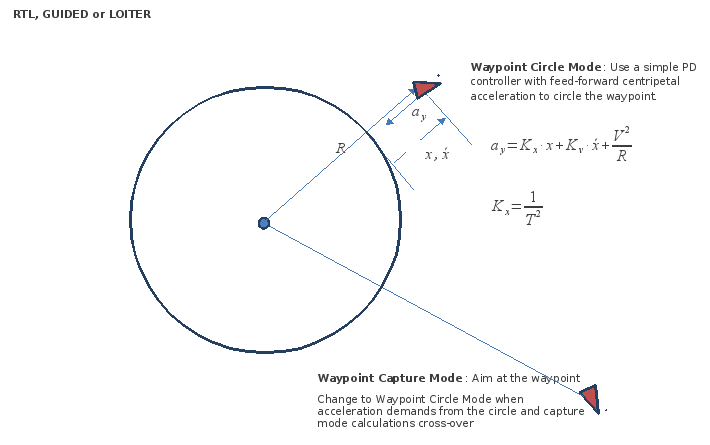
\includegraphics[width=0.8\linewidth]{figs/pd_loiter.png}	
  \caption{PD navigation controller, for circling waypoints. Source: ArduPilot}
  \label{fig:pd_loop}
\end{figure}


\subsection{Navigation: L1 Controller}

%S. Park, J. Deyst, and J. P. How, "A New Nonlinear Guidance Logic for
%Trajectory Tracking," Proceedings of the AIAA Guidance, Navigation and
%Control Conference, Aug 2004. AIAA-2004-4900.
%
%
Since a fixed-wing aircraft usually can't fly in-place, waypoints can be used in two general ways, the aircraft can fly around it in circles, or hit it and then follow to the next one.

In order to circle it, a L1 controller is used. L1 is an adaptative controller designed for trajectory following on aircraft\cite{Park04_GNC}. This technique provides better following of trajectories by taking advantage of the aircraft inertia and geometric properties of the desired path. The controller is briefly explained on Figure \ref{fig:l1_loop}.
%
%


\begin{figure}[H]
\centering
  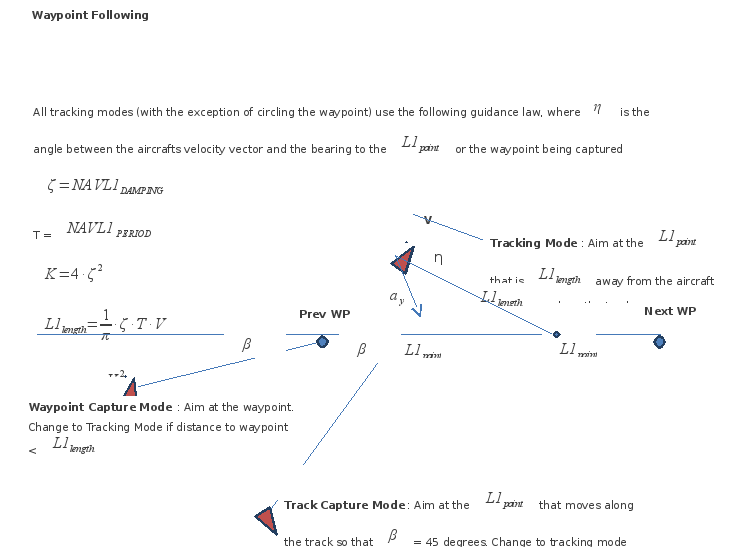
\includegraphics[width=0.8\linewidth]{figs/l1.png}	
  \caption{L1 navigation controller. Source: ArduPilot}
  \label{fig:l1_loop}
\end{figure}

\section{On VTOL Mode}
%
On the VTOL or multirotor mode, cascaded P/PID loops are used.
The inner loops control the angular speed, and the outer loops control the attitude, with the outermost loops controlling the altitude and position (again with the L1 controller). These controllers can be seen on Figure \ref{fig:copter_attitude_loops}.
\begin{figure}[H]
\centering
  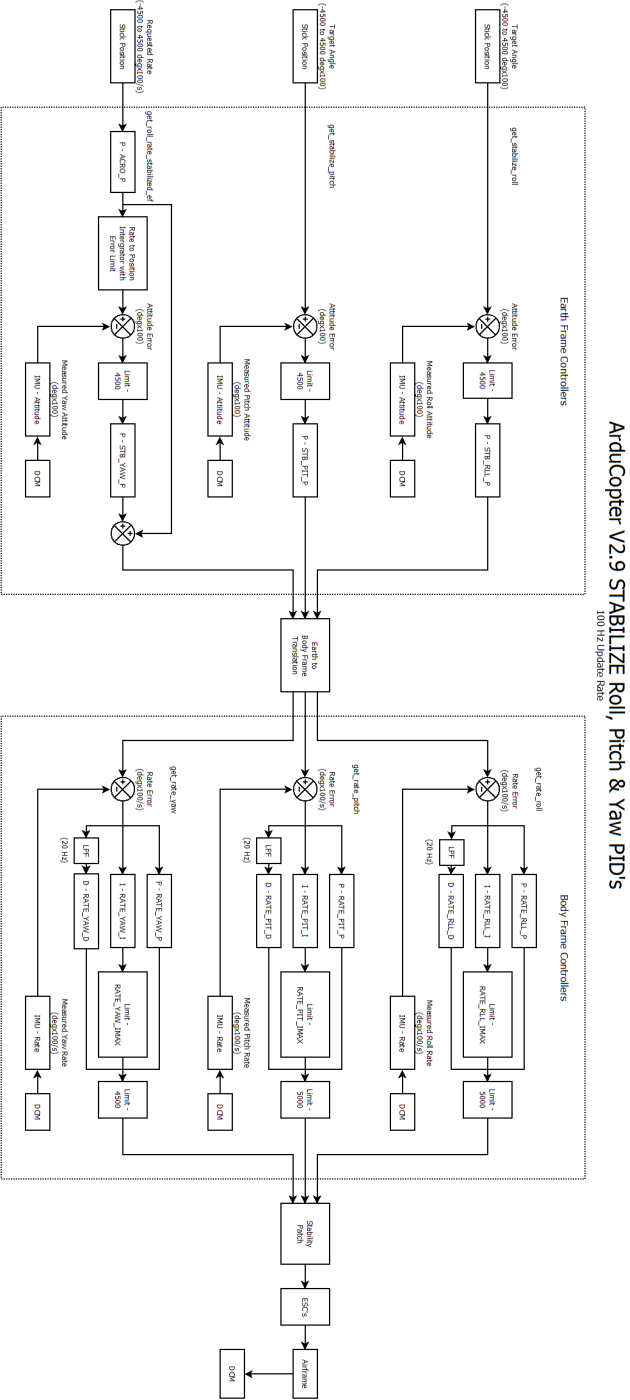
\includegraphics[width=0.65\linewidth]{figs/copterpids.png}
  \caption{Attitude controller. Source: ArduPilot}
  \label{fig:copter_attitude_loops}
\end{figure}

